\documentclass[a4paper,14pt]{article}

% --- Настройка шрифтов и локализации для XeLaTeX ---
\usepackage{fontspec}
\usepackage{xunicode}
\usepackage{xltxtra}
\usepackage{polyglossia}
\setmainlanguage{russian}
\setotherlanguage{english}
\defaultfontfeatures{Ligatures=TeX}
\setmainfont{Times New Roman}
\newfontfamily\cyrillicfont{Times New Roman}
\setmonofont{Courier New}
\newfontfamily\cyrillicfonttt{Courier New}

% --- Параметры страницы по ГОСТ (левое 3 см, правое 1 см, верхнее и нижнее по 2 см) ---
\usepackage[left=30mm, right=10mm, top=20mm, bottom=20mm]{geometry}

% --- Интервалы и абзацный отступ (1.25 см, 1.5 интервал) ---
\usepackage{indentfirst}
\setlength{\parindent}{1.25cm}
\usepackage{setspace}
\onehalfspacing

% --- Пакеты для таблиц, списков и графики ---
\usepackage{tabularx}
\usepackage{booktabs}
\usepackage{array}
\usepackage{enumitem}
\setlist{nosep, leftmargin=\parindent}
\usepackage{graphicx}

% --- Листинги SQL с корректным отображением пробелов в кириллице ---
\usepackage{listings}
\usepackage{xcolor}

\lstset{
    basicstyle=\ttfamily\footnotesize,
    columns=flexible,             % КЛЮЧЕВОЙ ПАРАМЕТР: отменяет схлопывание пробелов в XeLaTeX
    keepspaces=true,              % сохраняет исходные пробелы между словами
    breaklines=true,
    frame=single,
    tabsize=2,
    showstringspaces=false,
    keywordstyle=\bfseries\color{blue!70!black},
    commentstyle=\itshape\color{green!50!black},
    stringstyle=\color{red!60!black},
    numbers=none
}

% --- Оформление заголовков по стандарту ---
\usepackage{titlesec}
\titleformat{\section}[block]
  {\normalfont\bfseries\filright}
  {\hspace{1.25cm}\thesection\quad}
  {0pt}
  {\MakeUppercase}

\titleformat{\subsection}[block]
  {\normalfont\bfseries\filright}
  {\hspace{1.25cm}\thesubsection\quad}
  {0pt}
  {}

\titlespacing*{\section}{0pt}{18pt}{12pt}
\titlespacing*{\subsection}{0pt}{12pt}{6pt}

% Настройка подписей к рисункам и таблицам
\usepackage[tableposition=top,figureposition=bottom]{caption}
\DeclareCaptionLabelSeparator{emdash}{~---~}
\captionsetup[figure]{
  name={Рисунок},
  labelsep=emdash,
  font={small},
  justification=centering,
  singlelinecheck=true
}
\captionsetup[table]{
  name={Таблица},
  labelsep=emdash,
  font={small},
  justification=raggedright,
  singlelinecheck=false
}

% --- Отточие в содержании ---
\usepackage{tocloft}
\renewcommand{\cftsecleader}{\cftdotfill{\cftdotsep}}
\renewcommand{\cfttoctitlefont}{\hfill\bfseries\MakeUppercase}
\renewcommand{\cftaftertoctitle}{\hfill}

\begin{document}

% =========================================================================
% ТИТУЛЬНЫЙ ЛИСТ
% =========================================================================
\begin{titlepage}
    \centering
    {\small МИНИСТЕРСТВО НАУКИ И ВЫСШЕГО ОБРАЗОВАНИЯ РОССИЙСКОЙ ФЕДЕРАЦИИ}\\
    {\scriptsize \textbf{ФЕДЕРАЛЬНОЕ ГОСУДАРСТВЕННОЕ АВТОНОМНОЕ ОБРАЗОВАТЕЛЬНОЕ УЧРЕЖДЕНИЕ ВЫСШЕГО ОБРАЗОВАНИЯ}}\\
    {\bfseries «НАЦИОНАЛЬНЫЙ ИССЛЕДОВАТЕЛЬСКИЙ УНИВЕРСИТЕТ ИТМО»}\\[0.8cm]

    \textbf{Факультет безопасности информационных технологий}\\[0.6cm]

    \textbf{Направление подготовки: 10.03.01 Информационная безопасность} \\
    \textbf{Образовательная программа: «Технологии защиты информации»} \\[0.6cm]

    \textbf{Дисциплина:} \\
    \textit{\textbf{«Информационная безопасность баз данных»}} \\ [1.5cm]

    {\bfseries ОТЧЕТ ПО ЛАБОРАТОРНОЙ РАБОТЕ №2}\\
    \textit{{\bfseries «Реализация БД в рамках СУБД»}}\\[4cm]

    \begin{flushright}
        \textbf{Выполнил студент(ы):} \\ [0.5em]
        группа.поток ИББД 1.7 \\ [0.5em]
        Пахомов Владимир Юрьевич / \raisebox{-0.3\height}{
\includegraphics[width=1.3cm]{sign1.png}} \\
        {\scriptsize{\textit{ФИО \hspace{2cm} Подпись \hspace{0.3cm}}}} \\ [0.3cm]
        Сивков Иван Александрович / \raisebox{-0.4\height}{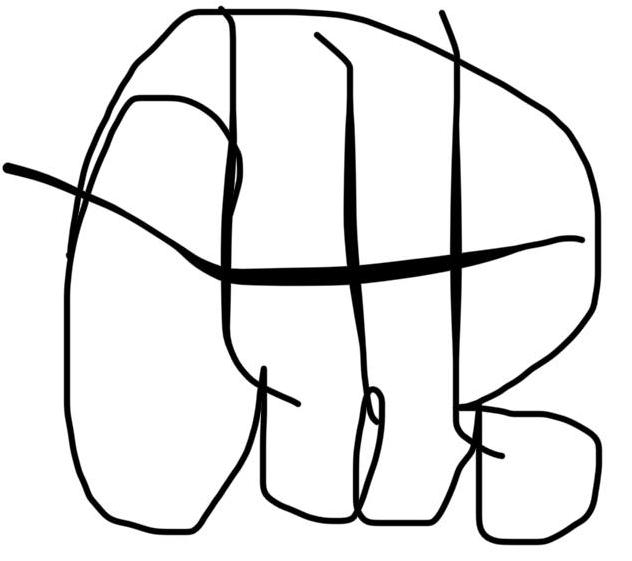
\includegraphics[width=1.1cm]{sign2.jpg}} \\
        {\scriptsize{\textit{ФИО \hspace{2cm} Подпись \hspace{0.3cm}}}} \\ [0.3cm]
        Булин Михаил Михайлович / \raisebox{-0.4\height}{
\includegraphics[width=1.3cm]{sign3.png}} \\
        {\scriptsize{\textit{ФИО \hspace{2cm} Подпись \hspace{0.3cm}}}} \\ [0.3cm]


        \textbf{Проверил:}\\ [0.5em]
        Ярцева Наталия Андреевна / \underline{\hspace{1.5cm}} \\
        {\scriptsize{\textit{ФИО \hspace{2cm} Подпись \hspace{1cm}}}} \\ [1.5cm]

        {\scriptsize \underline{\hspace{4cm}}} \\
        {\scriptsize \textit{Отметка о выполнении (один из вариантов: \\ отлично, хорошо, удовлетворительно, зачтено)}} \\
        {\scriptsize \underline{\hspace{4cm}}} \\
        {\scriptsize \textit{Дата \hspace{1.5cm}}}
    \end{flushright}

    \vfill
    Санкт-Петербург\\
    2026
\end{titlepage}

% =========================================================================
% СОДЕРЖАНИЕ
% =========================================================================
\newpage
\pagestyle{plain}
\setcounter{page}{2}

\begin{center}
    {\bfseries \MakeUppercase{Содержание}}
\end{center}
\vspace{-0.5cm}
\tableofcontents

% =========================================================================
% ВВЕДЕНИЕ
% =========================================================================
\newpage
\begin{center}
    {\bfseries \MakeUppercase{Введение}}
\end{center}
\addcontentsline{toc}{section}{ВВЕДЕНИЕ}

\textbf{Цель работы}: получение практических навыков работы с современными реляционными системами управления базами данных (СУБД), развертывания логической схемы отношений, обеспечения ссылочной целостности, индексно-ориентированной оптимизации запросов и программной реализации представлений (\textit{VIEW}).

В рамках данной работы выполняется физическая реализация базы данных «Информационная система морских контейнерных перевозок», спроектированной в лабораторной работе №1. Вся работа по созданию базы данных, генерации объектов схемы, конфигурированию ограничений, наполнению таблиц тестовыми данными и построению представлений выполняется с использованием консольного интерфейса терминала \texttt{psql}.

% =========================================================================
% 1. ВЫБОР СУБД И ИНСТРУМЕНТАРИЯ
% =========================================================================
\newpage
\section{Выбор СУБД и инструментария}

\subsection{Обоснование выбора СУБД PostgreSQL}
В качестве целевой системы управления базами данных выбрана свободно распространяемая объектно-реляционная СУБД PostgreSQL. Данный выбор обусловлен следующими ключевыми факторами:
\begin{itemize}
    \item полное соответствие стандартам SQL и строгая поддержка принципов ACID (атомарность, согласованность, изолированность, надежность);
    \item развитые механизмы обеспечения информационной безопасности, включающие дискреционный доступ (DAC), ролевую модель (RBAC), мандатную защиту на уровне строк (Row-Level Security, RLS) и встроенное шифрование;
    \item высокая производительность при обработке аналитических запросов с множественными соединениями таблиц (\textit{JOIN}) благодаря оптимизатору cost-based query planner;
    \item широкие возможности масштабирования и богатый набор встроенных механизмов индексации (B-Tree, Hash, GiST, GIN, BRIN).
\end{itemize}

\subsection{Обоснование выбора консольного клиента psql}
Для непосредственного администрирования и взаимодействия с сервером баз данных используется штатная интерактивная терминальная утилита \textbf{\texttt{psql}}.

Применение консольной утилиты вместо графических оболочек обосновано следующими преимуществами:
\begin{itemize}
    \item возможность полной автоматизации и воспроизводимости развертывания схемы базы данных через исполняемые SQL-скрипты;
    \item отсутствие накладных расходов на графическую подсистему и стабильная работа по защищенным протоколам удаленного доступа (SSH);
    \item прямой доступ к низкоуровневым сервисным метакомандам PostgreSQL (\texttt{\textbackslash d}, \texttt{\textbackslash dt}, \texttt{\textbackslash di}, \texttt{\textbackslash timing} и др.);
    \item соответствие регламентам безопасного администрирования промышленных серверов БД в изолированных сетевых контурах.
\end{itemize}

% =========================================================================
% 2. СОЗДАНИЕ БАЗЫ ДАННЫХ И СХЕМЫ ТАБЛИЦ
% =========================================================================
\newpage
\section{Создание базы данных и схемы таблиц}

\subsection{Создание базы данных в консоли psql}
Подключение к СУБД и инициализация новой базы данных выполняются следующими командами в терминале \texttt{psql}:

\begin{lstlisting}[language=SQL]
-- Подключение к экземпляру PostgreSQL
-- psql -U postgres -h localhost

CREATE DATABASE container_cargo_db
WITH 
    OWNER = postgres
    ENCODING = 'UTF8'
    LC_COLLATE = 'ru_RU.UTF-8'
    LC_CTYPE = 'ru_RU.UTF-8'
    TEMPLATE = template0;

-- Переключение на созданную базу данных
\c container_cargo_db
\end{lstlisting}

\subsection{Код создания отношений (таблиц)}
В соответствии со схемой, нормализованной в лабораторной работе №1, сформируем 7 базовых таблиц и 2 связующие таблицы отношений M:N.

\begin{lstlisting}[language=SQL]
-- 1. Таблица клиентов
CREATE TABLE clients (
    id SERIAL PRIMARY KEY,
    name VARCHAR(150) NOT NULL,
    email VARCHAR(100) NOT NULL UNIQUE,
    phone VARCHAR(30) NOT NULL,
    address VARCHAR(255) NOT NULL
);

-- 2. Таблица портов
CREATE TABLE ports (
    id SERIAL PRIMARY KEY,
    name VARCHAR(100) NOT NULL,
    country VARCHAR(100) NOT NULL,
    dock_count INTEGER NOT NULL CHECK (dock_count > 0),
    max_draft NUMERIC(4, 2) NOT NULL CHECK (max_draft > 0)
);

-- 3. Таблица судов
CREATE TABLE ships (
    id SERIAL PRIMARY KEY,
    name VARCHAR(100) NOT NULL,
    imo_number VARCHAR(20) NOT NULL UNIQUE,
    deadweight NUMERIC(10, 2) NOT NULL CHECK (deadweight > 0),
    year_built INTEGER NOT NULL CHECK (year_built >= 1950)
);

-- 4. Таблица контейнеров
CREATE TABLE containers (
    id SERIAL PRIMARY KEY,
    container_number VARCHAR(20) NOT NULL UNIQUE,
    type VARCHAR(50) NOT NULL,
    empty_weight NUMERIC(8, 2) NOT NULL CHECK (empty_weight > 0),
    capacity_volume NUMERIC(8, 2) NOT NULL CHECK (capacity_volume > 0)
);

-- 5. Таблица заказов
CREATE TABLE orders (
    id SERIAL PRIMARY KEY,
    client_id INTEGER NOT NULL,
    cargo_name VARCHAR(150) NOT NULL,
    cargo_weight NUMERIC(10, 2) NOT NULL CHECK (cargo_weight > 0),
    cargo_volume NUMERIC(10, 2) NOT NULL CHECK (cargo_volume > 0),
    total_price NUMERIC(12, 2) NOT NULL CHECK (total_price >= 0),
    created_at TIMESTAMP WITHOUT TIME ZONE DEFAULT CURRENT_TIMESTAMP
);

-- 6. Таблица морских рейсов
CREATE TABLE voyages (
    id SERIAL PRIMARY KEY,
    ship_id INTEGER NOT NULL,
    departure_port_id INTEGER NOT NULL,
    destination_port_id INTEGER NOT NULL,
    departure_date TIMESTAMP WITHOUT TIME ZONE NOT NULL,
    arrival_date TIMESTAMP WITHOUT TIME ZONE NOT NULL,
    status VARCHAR(30) NOT NULL DEFAULT 'Scheduled',
    CONSTRAINT chk_voyage_dates CHECK (arrival_date > departure_date),
    CONSTRAINT chk_voyage_ports CHECK (departure_port_id <> destination_port_id)
);

-- 7. Таблица счетов (инвойсов)
CREATE TABLE invoices (
    id SERIAL PRIMARY KEY,
    order_id INTEGER NOT NULL UNIQUE,
    invoice_number VARCHAR(50) NOT NULL UNIQUE,
    amount NUMERIC(12, 2) NOT NULL CHECK (amount >= 0),
    payment_status VARCHAR(30) NOT NULL DEFAULT 'Pending',
    issue_date DATE NOT NULL DEFAULT CURRENT_DATE
);

-- 8. Связующая таблица: Контейнеры заказа (M:N)
CREATE TABLE order_containers (
    id SERIAL PRIMARY KEY,
    order_id INTEGER NOT NULL,
    container_id INTEGER NOT NULL,
    seal_number VARCHAR(50) NOT NULL,
    gross_weight NUMERIC(10, 2) NOT NULL CHECK (gross_weight > 0),
    CONSTRAINT uq_order_container UNIQUE (order_id, container_id)
);

-- 9. Связующая таблица: Заказы рейса (M:N)
CREATE TABLE voyage_orders (
    id SERIAL PRIMARY KEY,
    voyage_id INTEGER NOT NULL,
    order_id INTEGER NOT NULL,
    loading_date TIMESTAMP WITHOUT TIME ZONE,
    discharge_date TIMESTAMP WITHOUT TIME ZONE,
    CONSTRAINT uq_voyage_order UNIQUE (voyage_id, order_id)
);
\end{lstlisting}

\subsection{Модификация структуры таблицы}
Продемонстрируем модификацию физической структуры существующей таблицы: добавим в отношение \textit{ships} атрибут государственной принадлежности флага судна (\textit{flag\_state}) и наложим проверочное ограничение.

\begin{lstlisting}[language=SQL]
-- Добавление нового атрибута для фиксации флага судна
ALTER TABLE ships 
ADD COLUMN flag_state VARCHAR(50) DEFAULT 'Россия';

-- Добавление проверочного ограничения длины строки
ALTER TABLE ships 
ADD CONSTRAINT chk_flag_state_length CHECK (LENGTH(flag_state) >= 2);
\end{lstlisting}

% =========================================================================
% 3. НАСТРОЙКА СВЯЗЕЙ И ИНДЕКСАЦИЯ ДАННЫХ
% =========================================================================
\newpage
\section{Настройка связей и индексация данных}

\subsection{Установление ссылочной целостности}
Для обеспечения строгой ссылочной целостности и предотвращения появления «висячих» ссылок добавим ограничения внешних ключей с каскадными политиками обновления и удаления.

\begin{lstlisting}[language=SQL]
-- Связь orders -> clients (1:M)
ALTER TABLE orders
ADD CONSTRAINT fk_orders_client FOREIGN KEY (client_id)
REFERENCES clients (id) ON UPDATE CASCADE ON DELETE RESTRICT;

-- Связь invoices -> orders (1:1)
ALTER TABLE invoices
ADD CONSTRAINT fk_invoices_order FOREIGN KEY (order_id)
REFERENCES orders (id) ON UPDATE CASCADE ON DELETE CASCADE;

-- Связи voyages -> ships, ports (1:M)
ALTER TABLE voyages
ADD CONSTRAINT fk_voyages_ship FOREIGN KEY (ship_id)
REFERENCES ships (id) ON UPDATE CASCADE ON DELETE RESTRICT,
ADD CONSTRAINT fk_voyages_dep_port FOREIGN KEY (departure_port_id)
REFERENCES ports (id) ON UPDATE CASCADE ON DELETE RESTRICT,
ADD CONSTRAINT fk_voyages_dest_port FOREIGN KEY (destination_port_id)
REFERENCES ports (id) ON UPDATE CASCADE ON DELETE RESTRICT;

-- Связи order_containers -> orders, containers (M:N)
ALTER TABLE order_containers
ADD CONSTRAINT fk_oc_order FOREIGN KEY (order_id)
REFERENCES orders (id) ON UPDATE CASCADE ON DELETE CASCADE,
ADD CONSTRAINT fk_oc_container FOREIGN KEY (container_id)
REFERENCES containers (id) ON UPDATE CASCADE ON DELETE RESTRICT;

-- Связи voyage_orders -> voyages, orders (M:N)
ALTER TABLE voyage_orders
ADD CONSTRAINT fk_vo_voyage FOREIGN KEY (voyage_id)
REFERENCES voyages (id) ON UPDATE CASCADE ON DELETE CASCADE,
ADD CONSTRAINT fk_vo_order FOREIGN KEY (order_id)
REFERENCES orders (id) ON UPDATE CASCADE ON DELETE CASCADE;
\end{lstlisting}

\subsection{Индексация атрибутов}
Для ускорения операций межтабличного соединения (\textit{JOIN}) и фильтрации данных (\textit{WHERE}) создадим индексные структуры типа B-Tree.

\begin{lstlisting}[language=SQL]
-- 1. Индексы под внешние ключи (ускорение JOIN)
CREATE INDEX idx_orders_client_id ON orders (client_id);
CREATE INDEX idx_voyages_ship_id ON voyages (ship_id);
CREATE INDEX idx_voyages_dep_port ON voyages (departure_port_id);
CREATE INDEX idx_voyages_dest_port ON voyages (destination_port_id);
CREATE INDEX idx_invoices_order_id ON invoices (order_id);
CREATE INDEX idx_oc_order_id ON order_containers (order_id);
CREATE INDEX idx_oc_container_id ON order_containers (container_id);
CREATE INDEX idx_vo_voyage_id ON voyage_orders (voyage_id);
CREATE INDEX idx_vo_order_id ON voyage_orders (order_id);

-- 2. Индексы под частый поиск и селективную фильтрацию (WHERE)
CREATE INDEX idx_clients_name ON clients (name);
CREATE INDEX idx_orders_cargo_name ON orders (cargo_name);
CREATE INDEX idx_voyages_status ON voyages (status);
CREATE INDEX idx_invoices_status ON invoices (payment_status);
CREATE INDEX idx_containers_type ON containers (type);
\end{lstlisting}

% =========================================================================
% 4. ЗАПОЛНЕНИЕ ТАБЛИЦ ТЕСТОВЫМИ ДАННЫМИ
% =========================================================================
\newpage
\section{Заполнение таблиц тестовыми данными}

Cгенерируем не менее 8 кортежей данных для каждой таблицы. Наполнение выполняется с соблюдением иерархии зависимостей (от независимых сущностей к подчиненным).

\subsection{Заполнение базовых сущностей}
\begin{lstlisting}[language=SQL]
-- Наполнение таблицы clients
INSERT INTO clients (name, email, phone, address) VALUES
('ООО БалтТрейд', 'info@balttrade.ru', '+7-812-555-0101', 'г. Санкт-Петербург, Морской пр., 12'),
('АО Восток-Логистик', 'contact@vostok.ru', '+7-423-222-3344', 'г. Владивосток, ул. Портовая, 5'),
('ПАО ТрансКонтейнер', 'order@transcont.ru', '+7-495-777-8899', 'г. Москва, ул. Новая Басманная, 2'),
('ООО Северный Путь', 'sp@nordway.com', '+7-818-245-1234', 'г. Архангельск, Набережная р. Двины, 18'),
('ИП Сидоров А.В.', 'sidorov@mail.ru', '+7-911-888-7766', 'г. Новороссийск, ул. Мира, 44'),
('ООО Глобал Импорт', 'import@globalimp.com', '+7-812-313-0099', 'г. Санкт-Петербург, Лиговский пр., 120'),
('ЗАО АгроЭкспорт', 'agro@export.ru', '+7-861-200-4567', 'г. Краснодар, ул. Красная, 78'),
('ООО ТехноПромХим', 'tph@chemtrade.ru', '+7-343-987-6543', 'г. Екатеринбург, ул. Ленина, 50');

-- Наполнение таблицы ports
INSERT INTO ports (name, country, dock_count, max_draft) VALUES
('Большой порт Санкт-Петербург', 'Россия', 16, 11.50),
('Порт Владивосток', 'Россия', 12, 12.00),
('Порт Новороссийск', 'Россия', 18, 13.50),
('Порт Шанхай', 'Китай', 45, 16.00),
('Порт Сингапур', 'Сингапур', 35, 15.50),
('Порт Пусан', 'Южная Корея', 28, 14.50),
('Порт Роттердам', 'Нидерланды', 30, 16.50),
('Порт Стамбул', 'Турция', 14, 12.50);

-- Наполнение таблицы ships
INSERT INTO ships (name, imo_number, deadweight, year_built, flag_state) VALUES
('Капитан Марков', 'IMO9123451', 52000.00, 2018, 'Россия'),
('Адмирал Ушаков', 'IMO9123452', 65000.00, 2020, 'Россия'),
('Балтийский Лидер', 'IMO9123453', 42000.00, 2015, 'Россия'),
('Pacific Voyager', 'IMO9123454', 80000.00, 2022, 'Панама'),
('Nordic Star', 'IMO9123455', 38000.00, 2012, 'Либерия'),
('Atlantic Pride', 'IMO9123456', 72000.00, 2019, 'Мальта'),
('Сибирь Экспресс', 'IMO9123457', 48000.00, 2021, 'Россия'),
('Oriental Dragon', 'IMO9123458', 85000.00, 2023, 'Сингапур');

-- Наполнение таблицы containers
INSERT INTO containers (container_number, type, empty_weight, capacity_volume) VALUES
('MSCU1234561', '40FT Standard', 3750.00, 67.70),
('MSCU1234562', '40FT High Cube', 3900.00, 76.40),
('TGHU7654321', '20FT Standard', 2230.00, 33.20),
('TGHU7654322', '20FT Reefer', 2950.00, 28.50),
('CMAU9988111', '40FT Reefer', 4400.00, 67.90),
('CMAU9988112', '20FT Standard', 2200.00, 33.10),
('HLXU5544331', '40FT High Cube', 3920.00, 76.30),
('HLXU5544332', '20FT Open Top', 2350.00, 32.50);
\end{lstlisting}

\subsection{Заполнение заказов, рейсов и подчиненных сущностей}
\begin{lstlisting}[language=SQL]
-- Наполнение таблицы orders
INSERT INTO orders (client_id, cargo_name, cargo_weight, cargo_volume, total_price) VALUES
(1, 'Электроника и микрочипы', 18500.00, 58.00, 450000.00),
(2, 'Текстильная продукция', 9200.00, 28.50, 210000.00),
(3, 'Автозапчасти и комплектующие', 24000.00, 65.00, 520000.00),
(4, 'Оборудование для пищевой пром.', 14300.00, 45.00, 380000.00),
(5, 'Медицинские препараты', 8400.00, 25.00, 310000.00),
(6, 'Бытовая техника', 19800.00, 62.00, 470000.00),
(7, 'Зерновые культуры в мешках', 26500.00, 70.00, 290000.00),
(8, 'Промышленная химия', 21500.00, 50.00, 430000.00);

-- Наполнение таблицы voyages
INSERT INTO voyages (ship_id, departure_port_id, destination_port_id, departure_date, arrival_date, status) VALUES
(1, 4, 1, '2026-03-01 08:00:00', '2026-03-25 18:00:00', 'Completed'),
(2, 1, 4, '2026-03-10 12:00:00', '2026-04-05 14:00:00', 'EnRoute'),
(3, 2, 6, '2026-03-15 09:00:00', '2026-03-20 16:00:00', 'Completed'),
(4, 5, 2, '2026-03-18 10:00:00', '2026-03-28 20:00:00', 'EnRoute'),
(5, 7, 1, '2026-03-22 06:00:00', '2026-03-30 15:00:00', 'Scheduled'),
(6, 3, 8, '2026-03-25 14:00:00', '2026-03-28 11:00:00', 'Scheduled'),
(7, 4, 2, '2026-04-01 08:00:00', '2026-04-12 18:00:00', 'Scheduled'),
(8, 6, 4, '2026-04-05 11:00:00', '2026-04-08 19:00:00', 'Scheduled');

-- Наполнение таблицы invoices
INSERT INTO invoices (order_id, invoice_number, amount, payment_status, issue_date) VALUES
(1, 'INV-2026-001', 450000.00, 'Paid', '2026-02-20'),
(2, 'INV-2026-002', 210000.00, 'Paid', '2026-02-22'),
(3, 'INV-2026-003', 520000.00, 'Pending', '2026-02-25'),
(4, 'INV-2026-004', 380000.00, 'Paid', '2026-03-01'),
(5, 'INV-2026-005', 310000.00, 'Pending', '2026-03-03'),
(6, 'INV-2026-006', 470000.00, 'Overdue', '2026-02-15'),
(7, 'INV-2026-007', 290000.00, 'Paid', '2026-03-05'),
(8, 'INV-2026-008', 430000.00, 'Pending', '2026-03-08');

-- Наполнение таблицы order_containers
INSERT INTO order_containers (order_id, container_id, seal_number, gross_weight) VALUES
(1, 1, 'SL-998811', 22250.00),
(2, 3, 'SL-445522', 11430.00),
(3, 2, 'SL-776633', 27900.00),
(4, 5, 'SL-112233', 18700.00),
(5, 4, 'SL-334455', 11350.00),
(6, 7, 'SL-556677', 23720.00),
(7, 8, 'SL-990011', 28850.00),
(8, 6, 'SL-887766', 23700.00);

-- Наполнение таблицы voyage_orders
INSERT INTO voyage_orders (voyage_id, order_id, loading_date, discharge_date) VALUES
(1, 1, '2026-03-01 10:30:00', '2026-03-25 16:00:00'),
(2, 2, '2026-03-10 14:00:00', NULL),
(3, 3, '2026-03-15 11:30:00', '2026-03-20 14:00:00'),
(4, 4, '2026-03-18 13:00:00', NULL),
(5, 5, NULL, NULL),
(6, 6, NULL, NULL),
(7, 7, NULL, NULL),
(8, 8, NULL, NULL);
\end{lstlisting}

% =========================================================================
% 5. СОЗДАНИЕ ПРЕДСТАВЛЕНИЙ (VIEW)
% =========================================================================
\newpage
\section{Создание представлений}

В соответствии с пунктом 5 лабораторной работы №1 создадим по 2 представления для каждого класса потребителей. Каждое представление агрегирует данные из двух и более связанных отношений.

\subsection{Представления для потребителя «Клиент / Грузоотправитель»}

\textbf{1. Представление \texttt{view\_client\_orders} («Реестр заказов и оплат»).}
\begin{lstlisting}[language=SQL]
CREATE OR REPLACE VIEW view_client_orders AS
SELECT 
    o.id AS order_id,
    o.client_id,
    o.cargo_name,
    o.total_price,
    i.invoice_number,
    i.payment_status,
    COUNT(oc.container_id) AS containers_count,
    COALESCE(SUM(oc.gross_weight), 0.00) AS actual_gross_weight
FROM orders o
LEFT JOIN invoices i ON o.id = i.order_id
LEFT JOIN order_containers oc ON o.id = oc.order_id
GROUP BY o.id, o.client_id, o.cargo_name, o.total_price, 
         i.invoice_number, i.payment_status;
\end{lstlisting}

\textbf{2. Представление \texttt{view\_client\_tracking} («Маршрутный трекинг груза»).}
\begin{lstlisting}[language=SQL]
CREATE OR REPLACE VIEW view_client_tracking AS
SELECT 
    o.id AS order_id,
    o.client_id,
    o.cargo_name,
    s.name AS vessel_name,
    p_dep.name AS port_of_loading,
    p_arr.name AS port_of_discharge,
    v.departure_date,
    v.arrival_date,
    v.status AS voyage_status
FROM orders o
JOIN voyage_orders vo ON o.id = vo.order_id
JOIN voyages v ON vo.voyage_id = v.id
JOIN ships s ON v.ship_id = s.id
JOIN ports p_dep ON v.departure_port_id = p_dep.id
JOIN ports p_arr ON v.destination_port_id = p_arr.id;
\end{lstlisting}

\subsection{Представления для потребителя «Диспетчер флота / Логист терминала»}

\textbf{1. Представление \texttt{view\_voyage\_manifest} («Судовой грузовой манифест»).}
\begin{lstlisting}[language=SQL]
CREATE OR REPLACE VIEW view_voyage_manifest AS
SELECT 
    v.id AS voyage_id,
    s.name AS ship_name,
    s.deadweight AS ship_capacity_tons,
    p1.name AS origin_port,
    p2.name AS destination_port,
    COUNT(vo.order_id) AS total_orders_assigned,
    COALESCE(SUM(o.cargo_weight), 0) / 1000.0 AS total_cargo_tons
FROM voyages v
JOIN ships s ON v.ship_id = s.id
JOIN ports p1 ON v.departure_port_id = p1.id
JOIN ports p2 ON v.destination_port_id = p2.id
LEFT JOIN voyage_orders vo ON v.id = vo.voyage_id
LEFT JOIN orders o ON vo.order_id = o.id
GROUP BY v.id, s.name, s.deadweight, p1.name, p2.name;
\end{lstlisting}

\textbf{2. Представление \texttt{view\_container\_safety\_audit} («Ведомость контроля веса и пломб»).}
\begin{lstlisting}[language=SQL]
CREATE OR REPLACE VIEW view_container_safety_audit AS
SELECT 
    c.container_number,
    c.type AS container_type,
    c.empty_weight AS tare_weight,
    oc.seal_number,
    oc.gross_weight,
    (oc.gross_weight - c.empty_weight) AS net_cargo_weight,
    o.id AS order_id,
    cl.name AS shipper_name
FROM order_containers oc
JOIN containers c ON oc.container_id = c.id
JOIN orders o ON oc.order_id = o.id
JOIN clients cl ON o.client_id = cl.id;
\end{lstlisting}

% =========================================================================
% ЗАКЛЮЧЕНИЕ
% =========================================================================
\newpage
\begin{center}
    {\bfseries \MakeUppercase{Заключение}}
\end{center}
\addcontentsline{toc}{section}{ЗАКЛЮЧЕНИЕ}

В ходе выполнения лабораторной работы была полностью реализована реляционная база данных для «Информационной системы контейнерных перевозок» в среде PostgreSQL с использованием консольного интерфейса \texttt{psql}.

В процессе выполнения работы были решены следующие задачи:
\begin{enumerate}
    \item Обоснован выбор СУБД PostgreSQL и терминального клиента \texttt{psql} с точки зрения надежности, соответствия ACID и практической информационной безопасности.
    \item Написаны и успешно применены скрипты генерации 9 таблиц (7 базовых отношений и 2 связующих для реализации кардинальности M:N).
    \item Продемонстрировано использование команд изменения физической структуры отношений (\textit{ALTER TABLE}) для добавления новых колонок и ограничений целостности.
    \item Настроена ссылочная целостность с помощью первичных и внешних ключей (\textit{PK, FK, CHECK, UNIQUE, NOT NULL}).
    \item Проведена индексация ключевых полей для ускорения операций объединения (\textit{JOIN}) и фильтрации (\textit{WHERE}).
    \item Все таблицы наполнены осмысленными тестовыми данными.
    \item Реализованы 4 многотабличных представления (\textit{VIEW}), обеспечивающих ролевой доступ к данным для клиентов-грузоотправителей и логистов терминала.
\end{enumerate}

Разработанная база данных находится в работоспособном состоянии, готова к проведению тестов безопасности и разграничению прав доступа на уровне ролей СУБД.

\end{document}